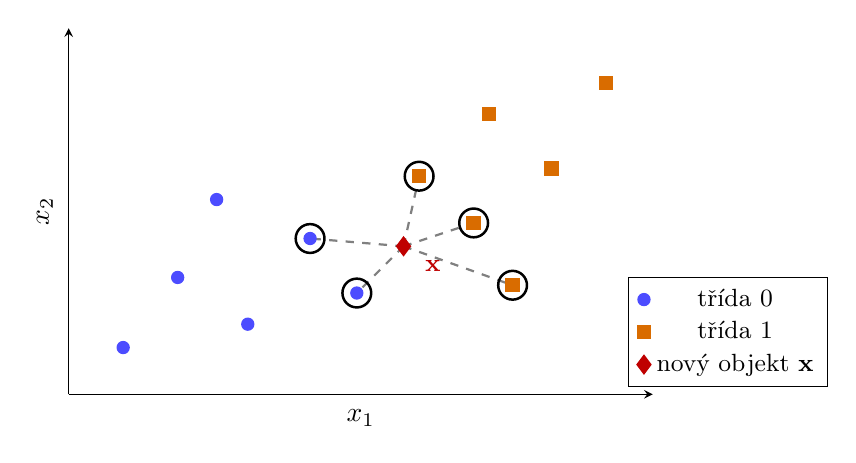
\begin{tikzpicture}
    \begin{axis}[
        width=9cm,
        height=7.8cm,
        xmin=0.5, xmax=8,
        ymin=0.5, ymax=5.2,
        axis lines=left,
        axis equal image,
        xlabel={$x_1$},
        ylabel={$x_2$},
        xtick=\empty,
        ytick=\empty,
        clip=false,
        legend style={
            at={(1.3,0.02)},
            anchor=south east,
            font=\small
        }
    ]

        % třída 0
        \addplot[
            only marks,
            mark=*,
            mark size=2.2pt,
            blue!70
        ] coordinates {
            (1.2,1.1)
            (1.9,2.0)
            (2.8,1.4)
            (3.6,2.5)
            (4.2,1.8)
            (2.4,3.0)
        };
        \addlegendentry{třída~\(0\)}

        % třída 1
        \addplot[
            only marks,
            mark=square*,
            mark size=2.4pt,
            orange!85!black
        ] coordinates {
            (5.0,3.3)
            (5.7,2.7)
            (5.9,4.1)
            (6.7,3.4)
            (7.4,4.5)
            (6.2,1.9)
        };
        \addlegendentry{třída~\(1\)}

        % nový objekt
        \addplot[
            only marks,
            mark=diamond*,
            mark size=3.4pt,
            red!75!black
        ] coordinates {
            (4.8,2.4)
        };
        \addlegendentry{nový objekt \(\mathbf{x}\)}

        % zvýraznění 5 nejbližších sousedů
        \addplot[
            only marks,
            mark=o,
            mark size=5.2pt,
            black,
            line width=0.9pt
        ] coordinates {
            (4.2,1.8)
            (3.6,2.5)
            (5.0,3.3)
            (5.7,2.7)
            (6.2,1.9)
        };

        % spojnice k 5 nejbližším sousedům
        \draw[dashed, thick, gray]
            (axis cs:4.8,2.4) -- (axis cs:4.2,1.8);
        \draw[dashed, thick, gray]
            (axis cs:4.8,2.4) -- (axis cs:3.6,2.5);
        \draw[dashed, thick, gray]
            (axis cs:4.8,2.4) -- (axis cs:5.0,3.3);
        \draw[dashed, thick, gray]
            (axis cs:4.8,2.4) -- (axis cs:5.7,2.7);
        \draw[dashed, thick, gray]
            (axis cs:4.8,2.4) -- (axis cs:6.2,1.9);

        % popisek nového objektu
        \node[
            font=\small,
            red!75!black,
            anchor=west
        ] at (axis cs:4.95,2.15) {\(\mathbf{x}\)};

    \end{axis}
\end{tikzpicture}
